% Бүлэг 3

\chapter{Системийн зохиомж} % Зарим нэг зөвлөмж
\label{Chapter3} % Энэ бүлэг рүү ишлэл хийх бол \ref{Chapter2} командыг ашигла 

	\section{Өгөгдлийн ерөнхий схем}
		\begin{figure}[ht]
			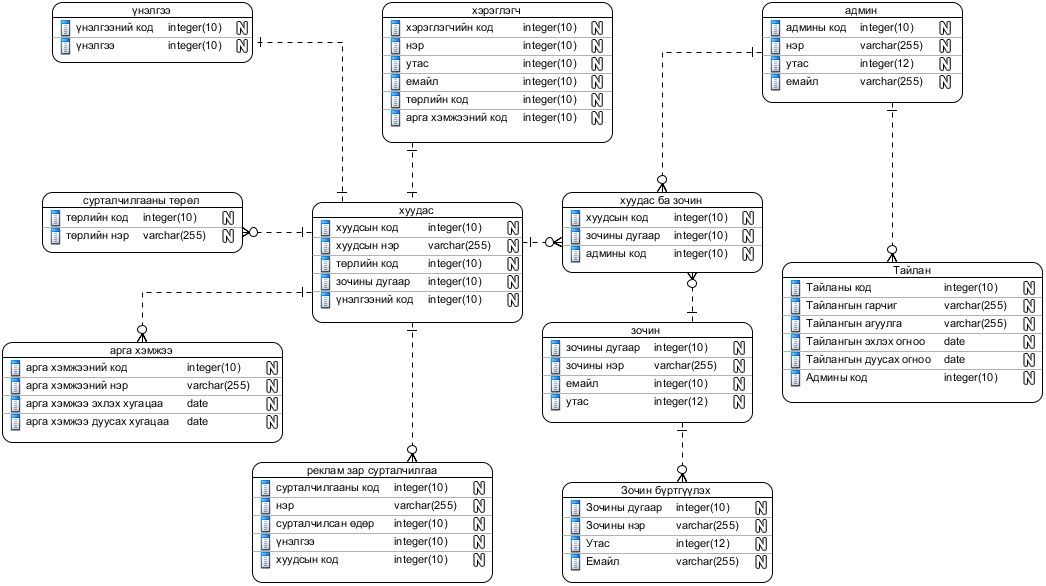
\includegraphics[width=27cm,angle=90,scale=0.7]{Diagrams/Entity}
			\caption[Өгөгдлийн ерөнхий схем]{Өгөгдлийн ерөнхий схем}
			\label{text}
		\end{figure}

\section{Класс диаграм}
	\begin{figure}[ht]
		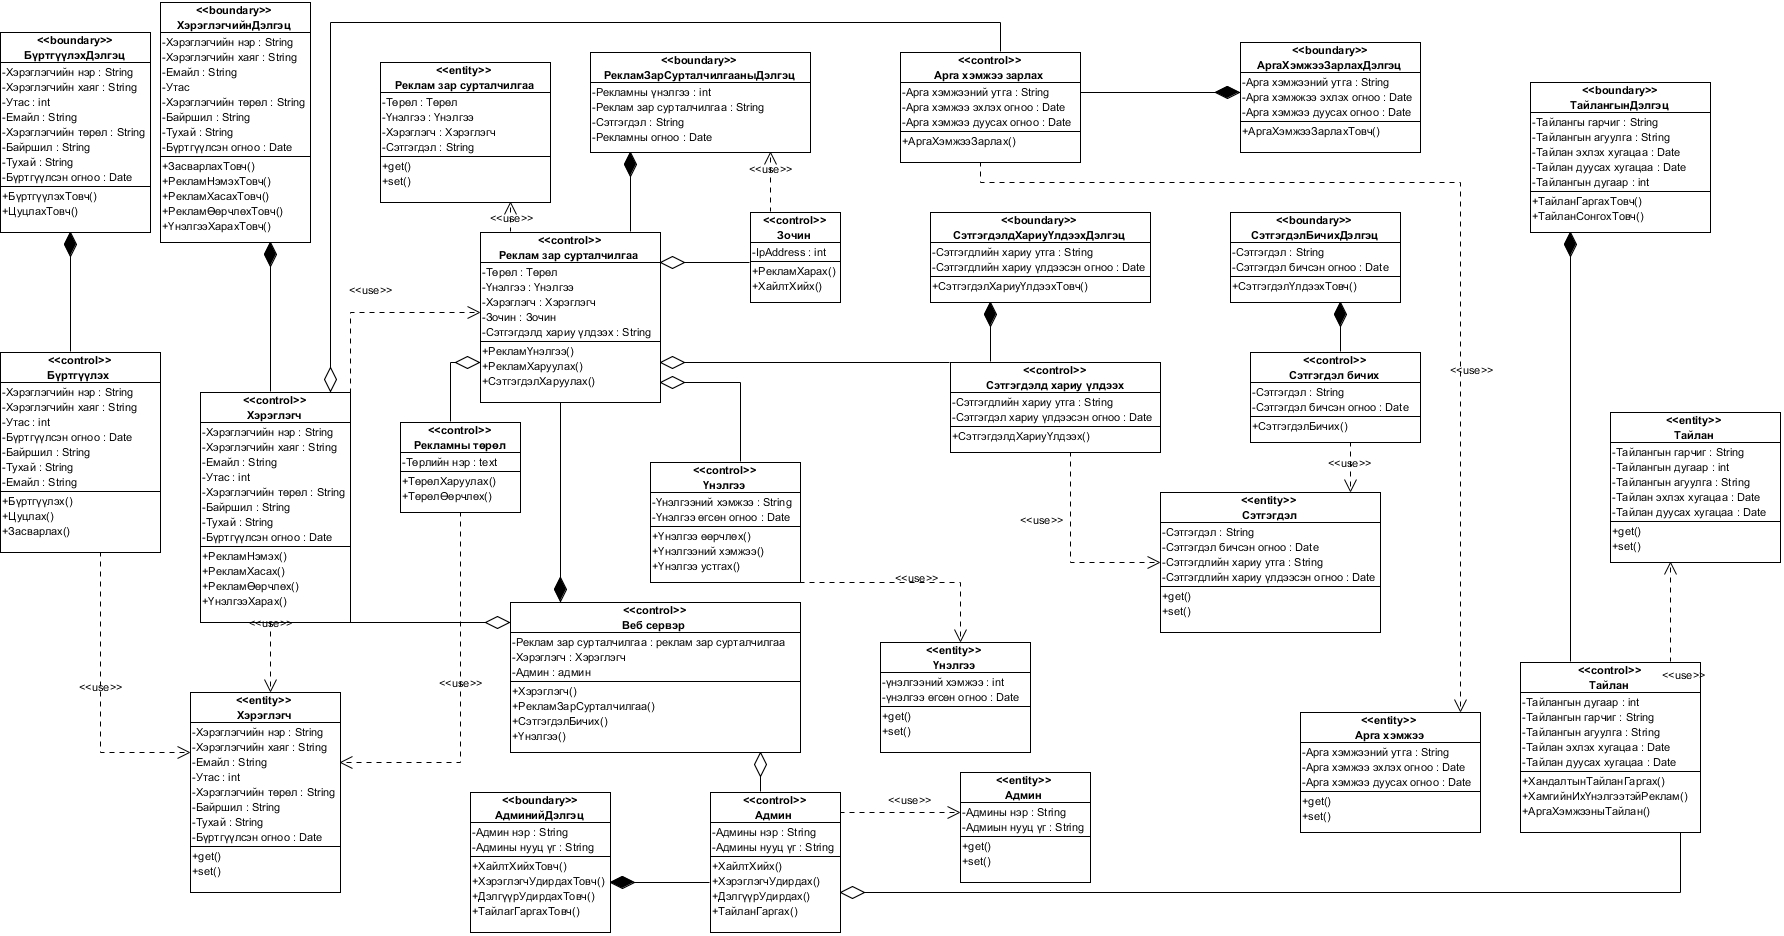
\includegraphics[angle=90,scale=0.34]{Diagrams/z_class}
		\caption[Зохиомжийн шатны класс диаграм]{Зохиомжийн шатны класс диаграм}
		\label{text}
	\end{figure}
\section{Дарааллын диаграм }
	\begin{figure}[ht]
		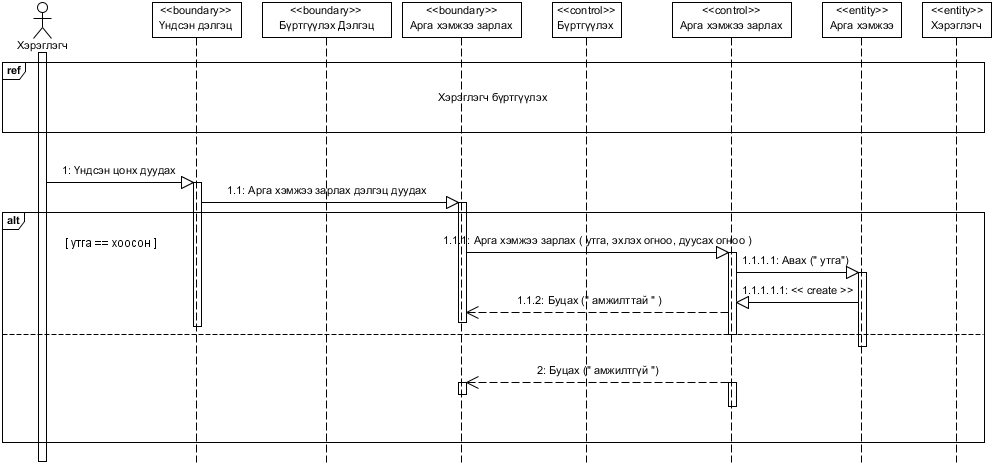
\includegraphics[scale=0.48]{Diagrams/event_s}
		\caption[Арга хэмжээ зарлах дарааллын диаграм]{Арга хэмжээ зарлах дарааллын диаграм}
		\label{text}
	\end{figure}

	\begin{figure}[ht]
		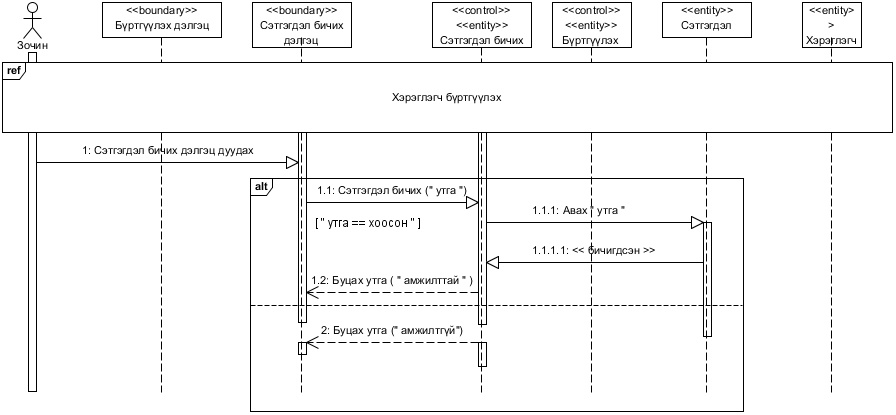
\includegraphics[scale=0.53]{Diagrams/comment_s}
		\caption[Сэтгэгдэл бичих дарааллын диаграм]{Сэтгэгдэл бичих дарааллын диаграм}
		\label{text}
	\end{figure}
	
	\begin{figure}[ht]
		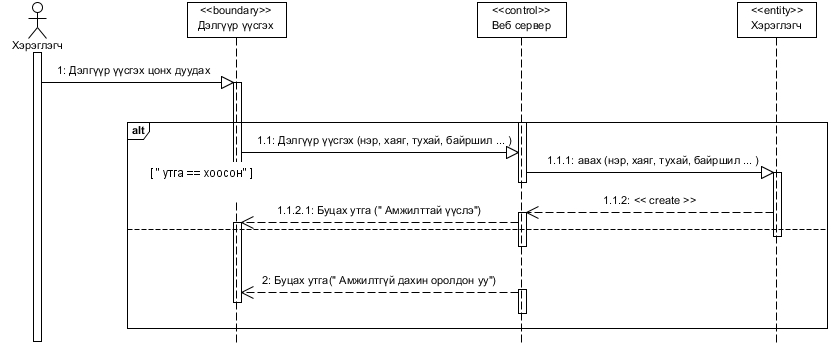
\includegraphics[scale=0.55]{Diagrams/create_s}
		\caption[Дэлгүүр үүсгэх дарааллын диаграм]{Дэлгүүр үүсгэх дарааллын диаграм}
		\label{text}
	\end{figure}


\section{Төлөвийн диаграм }
	\begin{figure}[ht]

		\includegraphics[scale=0.55]{Diagrams/state}
		\caption[Реклам зар сурталчилгаа удирдах төлөвийн диаграм]{Реклам зар сурталчилгаа удирдах төлөвийн диаграм}
		\label{text}
	\end{figure}

\section{Хэрэглэгчийн интерфейс }
	
\section{Тайлан, статистик үзүүлэлтийн загвар }
	
\section{Бүлгийн дүгнэлт}
	Зохиомжийн хэсэгт өгөгдлийн ерөнхий схем болон өмнөх шинжилгээний класс диаграм дээр үндэслэн зохиомжийн класс диаграм, дарааллын диаграмуудыг гаргасан. Хамгийн гол төлөвийн диаграмыг бас давхар гаргаж өгсөн байгаа. Бусад ижил төстэй томоохон сайтуудаас жишээ авч вебийн туршилтын загварыг гаргасан байгаа
\section{Ерөнхий дүгнэлт}
	Өнөө үед интернэтийн орчинд ажил, үйлчилгээгээ явуулах хувь хүн болон аж ахуйн нэгж албан байгууллагууд хурдацтай өсөн нэмэгдсэн билээ. Үүнийг ажиглан реклам зар сурталчилгааг интернэт дамжуулан хэрэглэгчид хүргэх нь одоогийн нийгэмд хамгийн зөв арга хэлбэр болоод байна. Энэхүү вебийг хийхэд дараах ажлуудыг хийж гүйцэтгэлээ:
	-	Тухайн вебийн талаар судалгаа явсан
	-	CodeIgniter framework –ийн судалгаа хийсэн
	-	Өгөгдлийн сан болон вебийн дотоод үйл ажиллагааг дүрслэн гаргасан
	-	Код бичих орчиноо бэлдэх, судалгаа шинжилгээ хийсэн
	
